\documentclass[12;pt,t]{beamer} % beamer - typ/šablona prezentace

\usepackage[czech]{babel} % nastavuje české popisky např. u obsahu, referencí, tabulek, obázků 
\usepackage[utf8]{inputenc} % použito UTF8 kvůli češtině (zvládá prakticky všechny jazyky na světě)
\usepackage[T1]{fontenc}

\usepackage{lmodern}
%\usepackage{datetime}
\usepackage{amssymb} % podpůrná knihovna pro matematické symboly
\usepackage{enumerate} % umožňuje širší možnosti nastavení enumerate

\usepackage{graphicx} % vkládání obrázků
\usepackage{hologo} % logo BibTeX

\usepackage{multicol} % pro praci s více sloupci

\usepackage{xcolor}
\usepackage{listings}

\lstset{basicstyle=\footnotesize\ttfamily,
  showstringspaces=false,
  commentstyle=\color{red},
  keywordstyle=\color{blue},
  escapeinside={(*@}{@*)},
  breaklines=true,
  extendedchars=true,
  inputencoding=utf8
}

\lstdefinelanguage{bettertex}{%
  language     = tex,
  morekeywords = {begin,hline},
}

% pro pěkné zobrazení zdroje obrázků
\definecolor{sourcesclr}{rgb}{.38,.38,.38}
\newcommand{\srctext}[1]{{\fontsize{7}{9}\selectfont\textcolor{sourcesclr}{#1}}}

% Themes: http://www.hartwork.org/beamer-theme-matrix/
\mode<presentation>{\usetheme{Madrid}}
\usecolortheme{beaver}
\beamertemplatenavigationsymbolsempty 
\setbeamertemplate{title page}[default][colsep=0bp,rounded=true]
\setbeamertemplate{itemize items}{-} %$\circ$
\setbeamercolor*{item}{fg=black}
\setbeamertemplate{enumerate item}[default]


\author{Jaroslav Páral}
\institute[paral.jarek@gmail.com]{FI MUNI: F5090\\[0.5cm]}
\title{Elektronické součástky a plošné spoje}


\begin{document}

\frame{\titlepage}

\begin{frame}
    \frametitle{Součástky - THT a SMD}
    	\begin{figure}[H]
            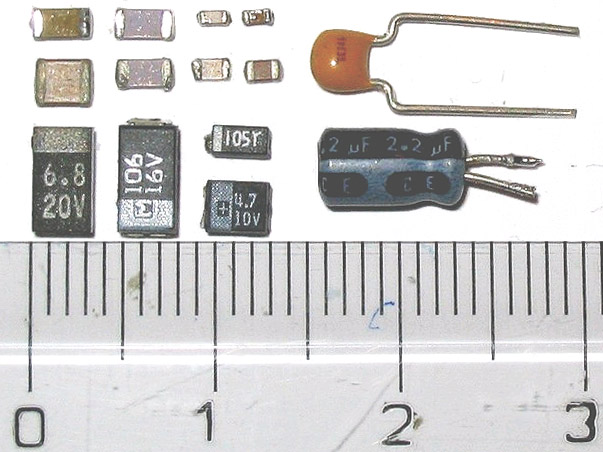
\includegraphics[width=0.75\textwidth]{img/Photo-SMDcapacitors.jpg}
            %\caption{Harvesting of the solar energy}
    	\end{figure}
    	    \srctext{Zdroj obrázku: \url{https://commons.wikimedia.org/wiki/File:Photo-SMDcapacitors.jpg}}
\end{frame}

\begin{frame}
\frametitle{Součástky - THT (Through-hole technology) - rezistor}
\begin{figure}[H]
	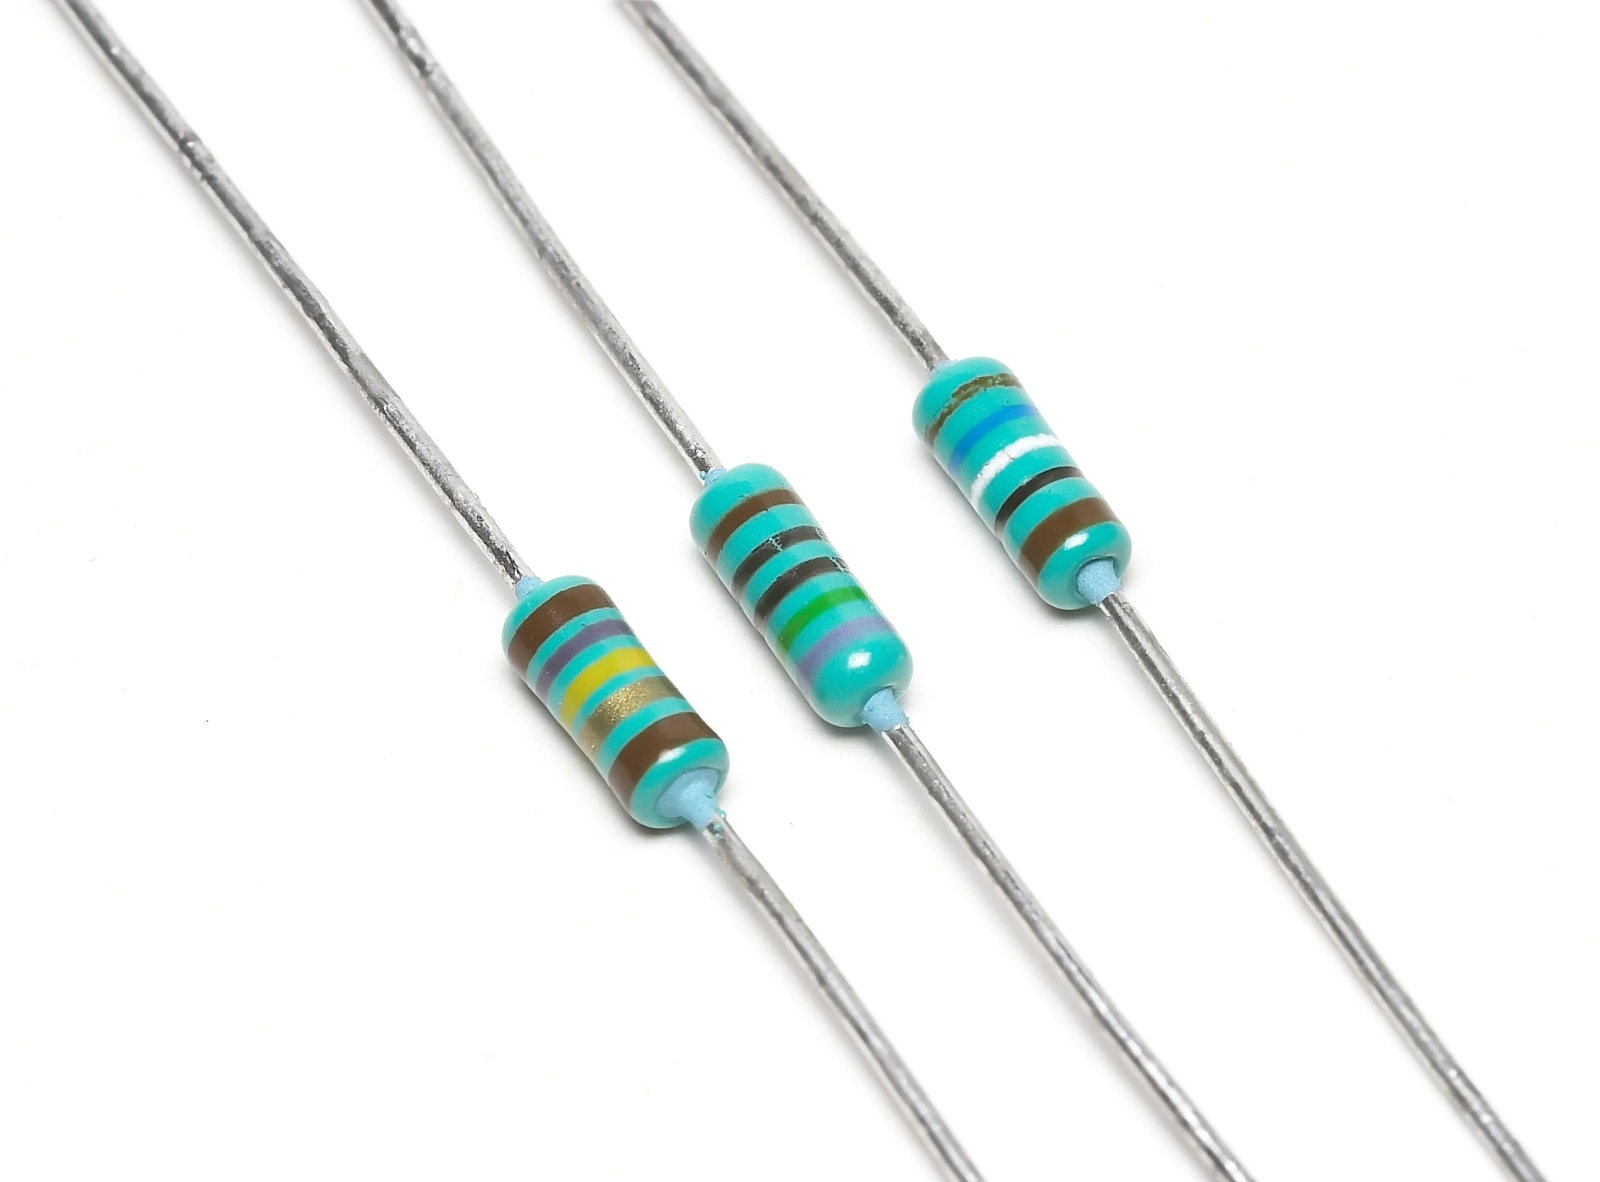
\includegraphics[width=0.75\textwidth]{img/3_Resistors.jpg}
	%\caption{Harvesting of the solar energy}
\end{figure}
\srctext{Zdroj obrázku: \url{
	https://commons.wikimedia.org/wiki/File:3_Resistors.jpg}}
\end{frame}

\begin{frame}
\frametitle{Součástky - THT (Through-hole technology) - kondenzátor}
\begin{figure}[H]
	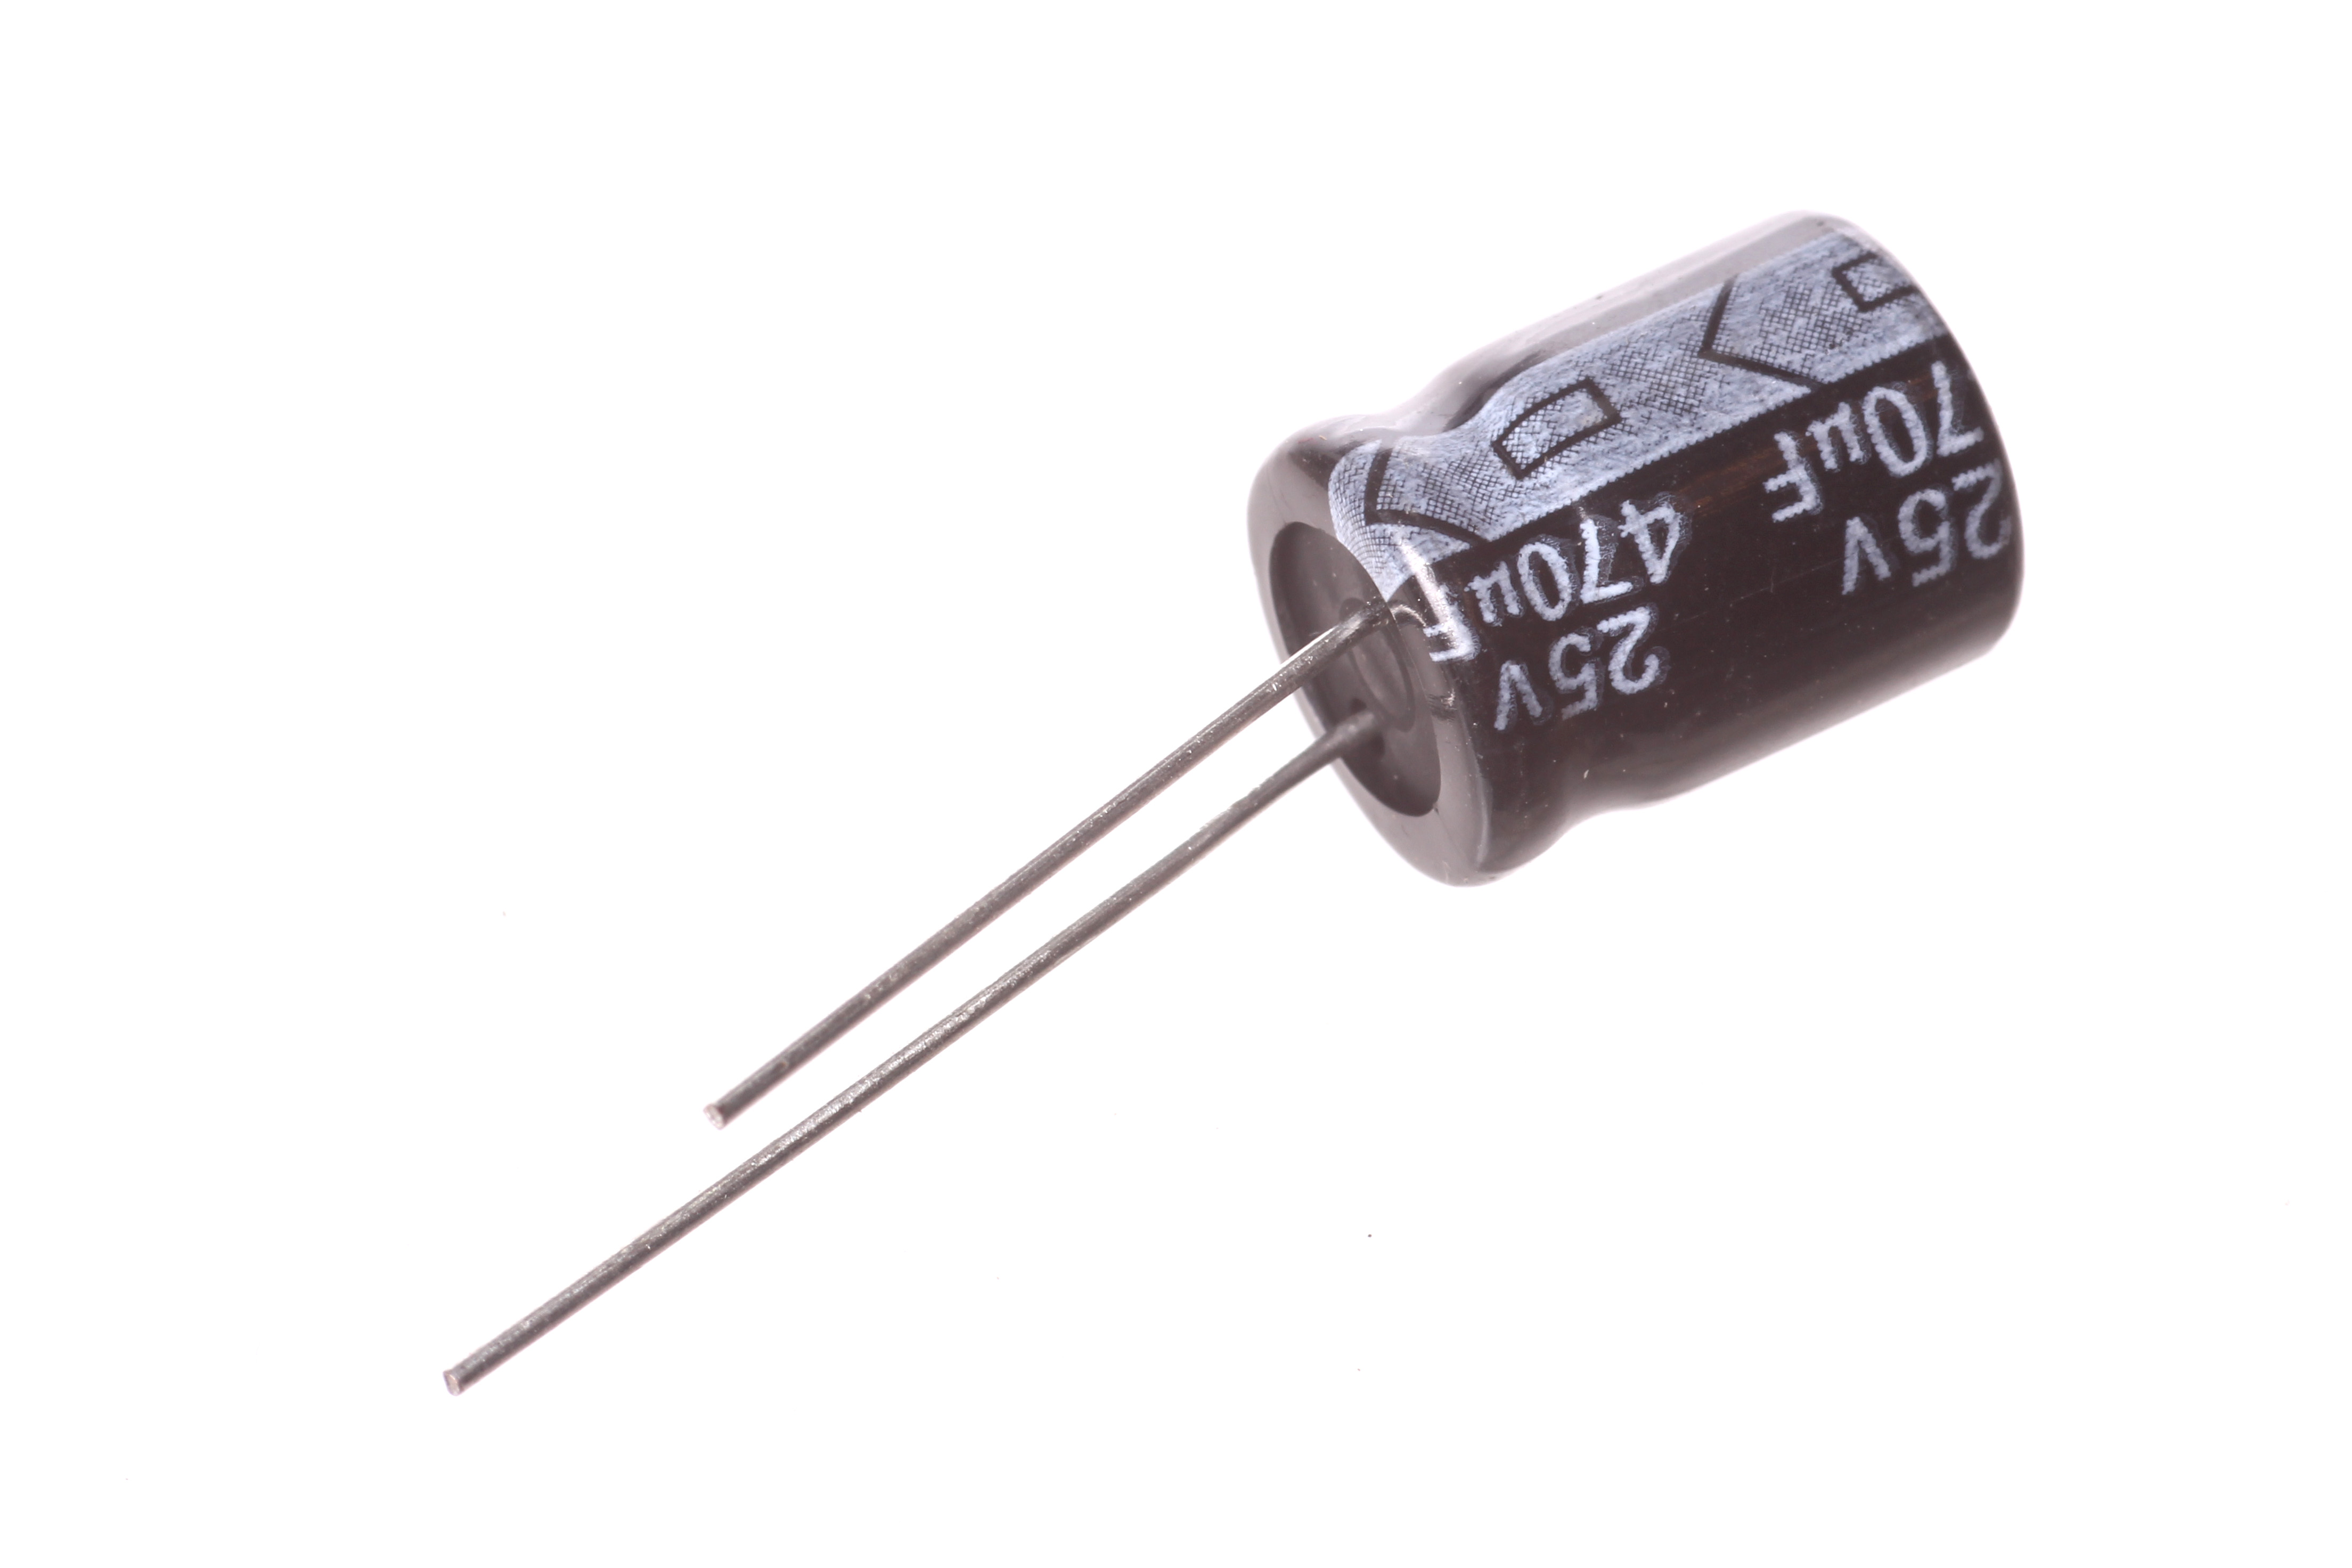
\includegraphics[width=0.8\textwidth]{img/CAPE-TH-X-UF470-VA_(16236695369).jpg}
	%\caption{Harvesting of the solar energy}
\end{figure}
\srctext{Zdroj obrázku: \url{
		https://commons.wikimedia.org/wiki/File:CAPE-TH-X-UF470-VA_(16236695369).jpg}}
\end{frame}

\begin{frame}
\frametitle{Součástky - THT (Through-hole technology) - IC}
\begin{figure}[H]
	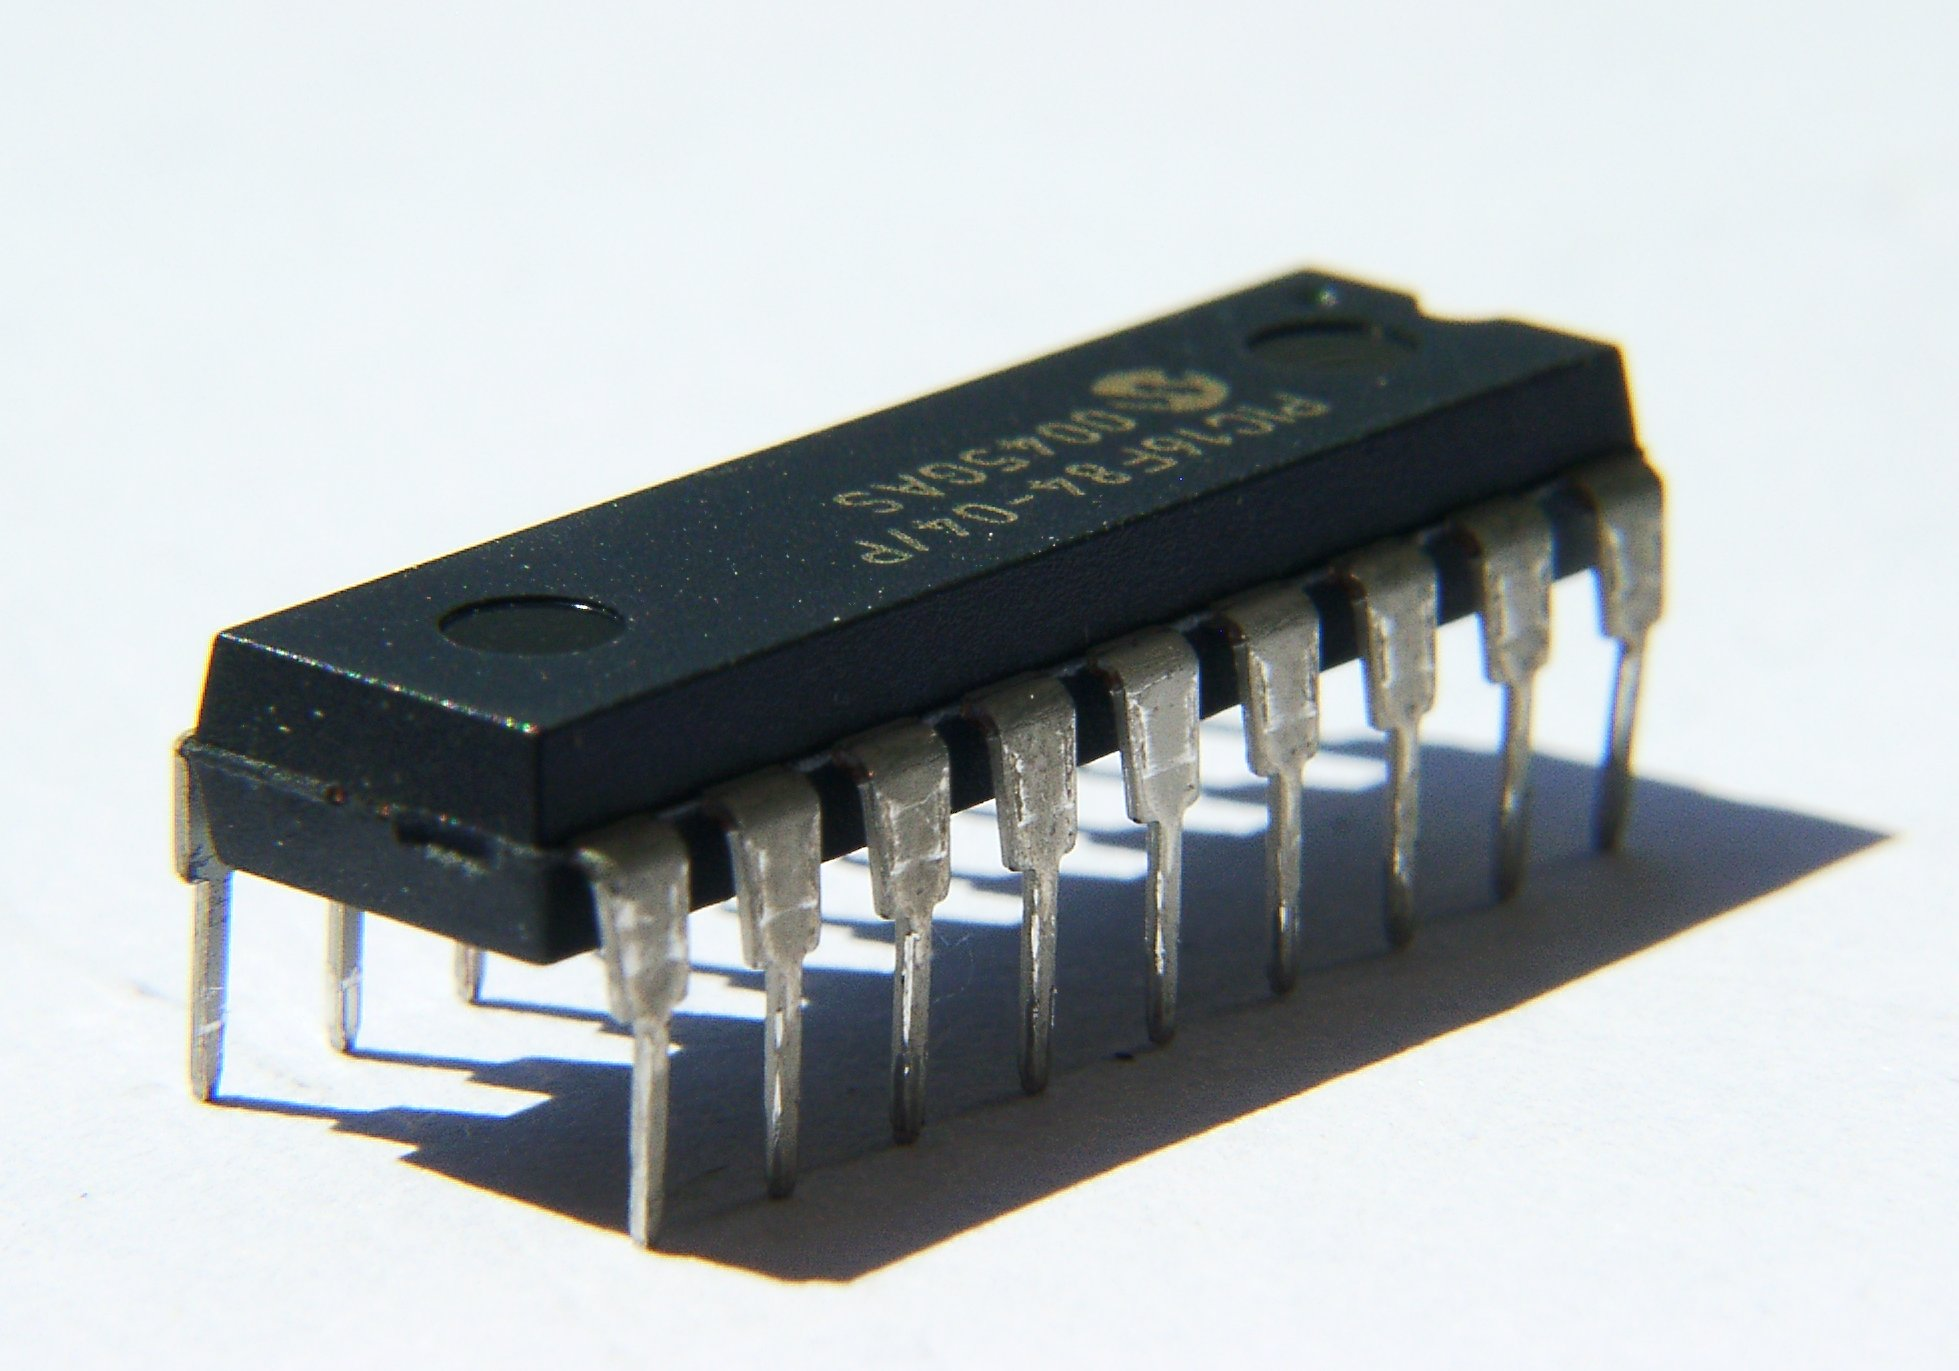
\includegraphics[width=0.8\textwidth]{img/Integrated_Circuit_THT.jpg}
	%\caption{Harvesting of the solar energy}
\end{figure}
\srctext{Zdroj obrázku: \url{https://commons.wikimedia.org/wiki/File:Integrated_Circuit.jpg}}
\end{frame}

\begin{frame}
\frametitle{Součástky - SMD (surface mount device) - rezistor}    	
\begin{figure}[H]
	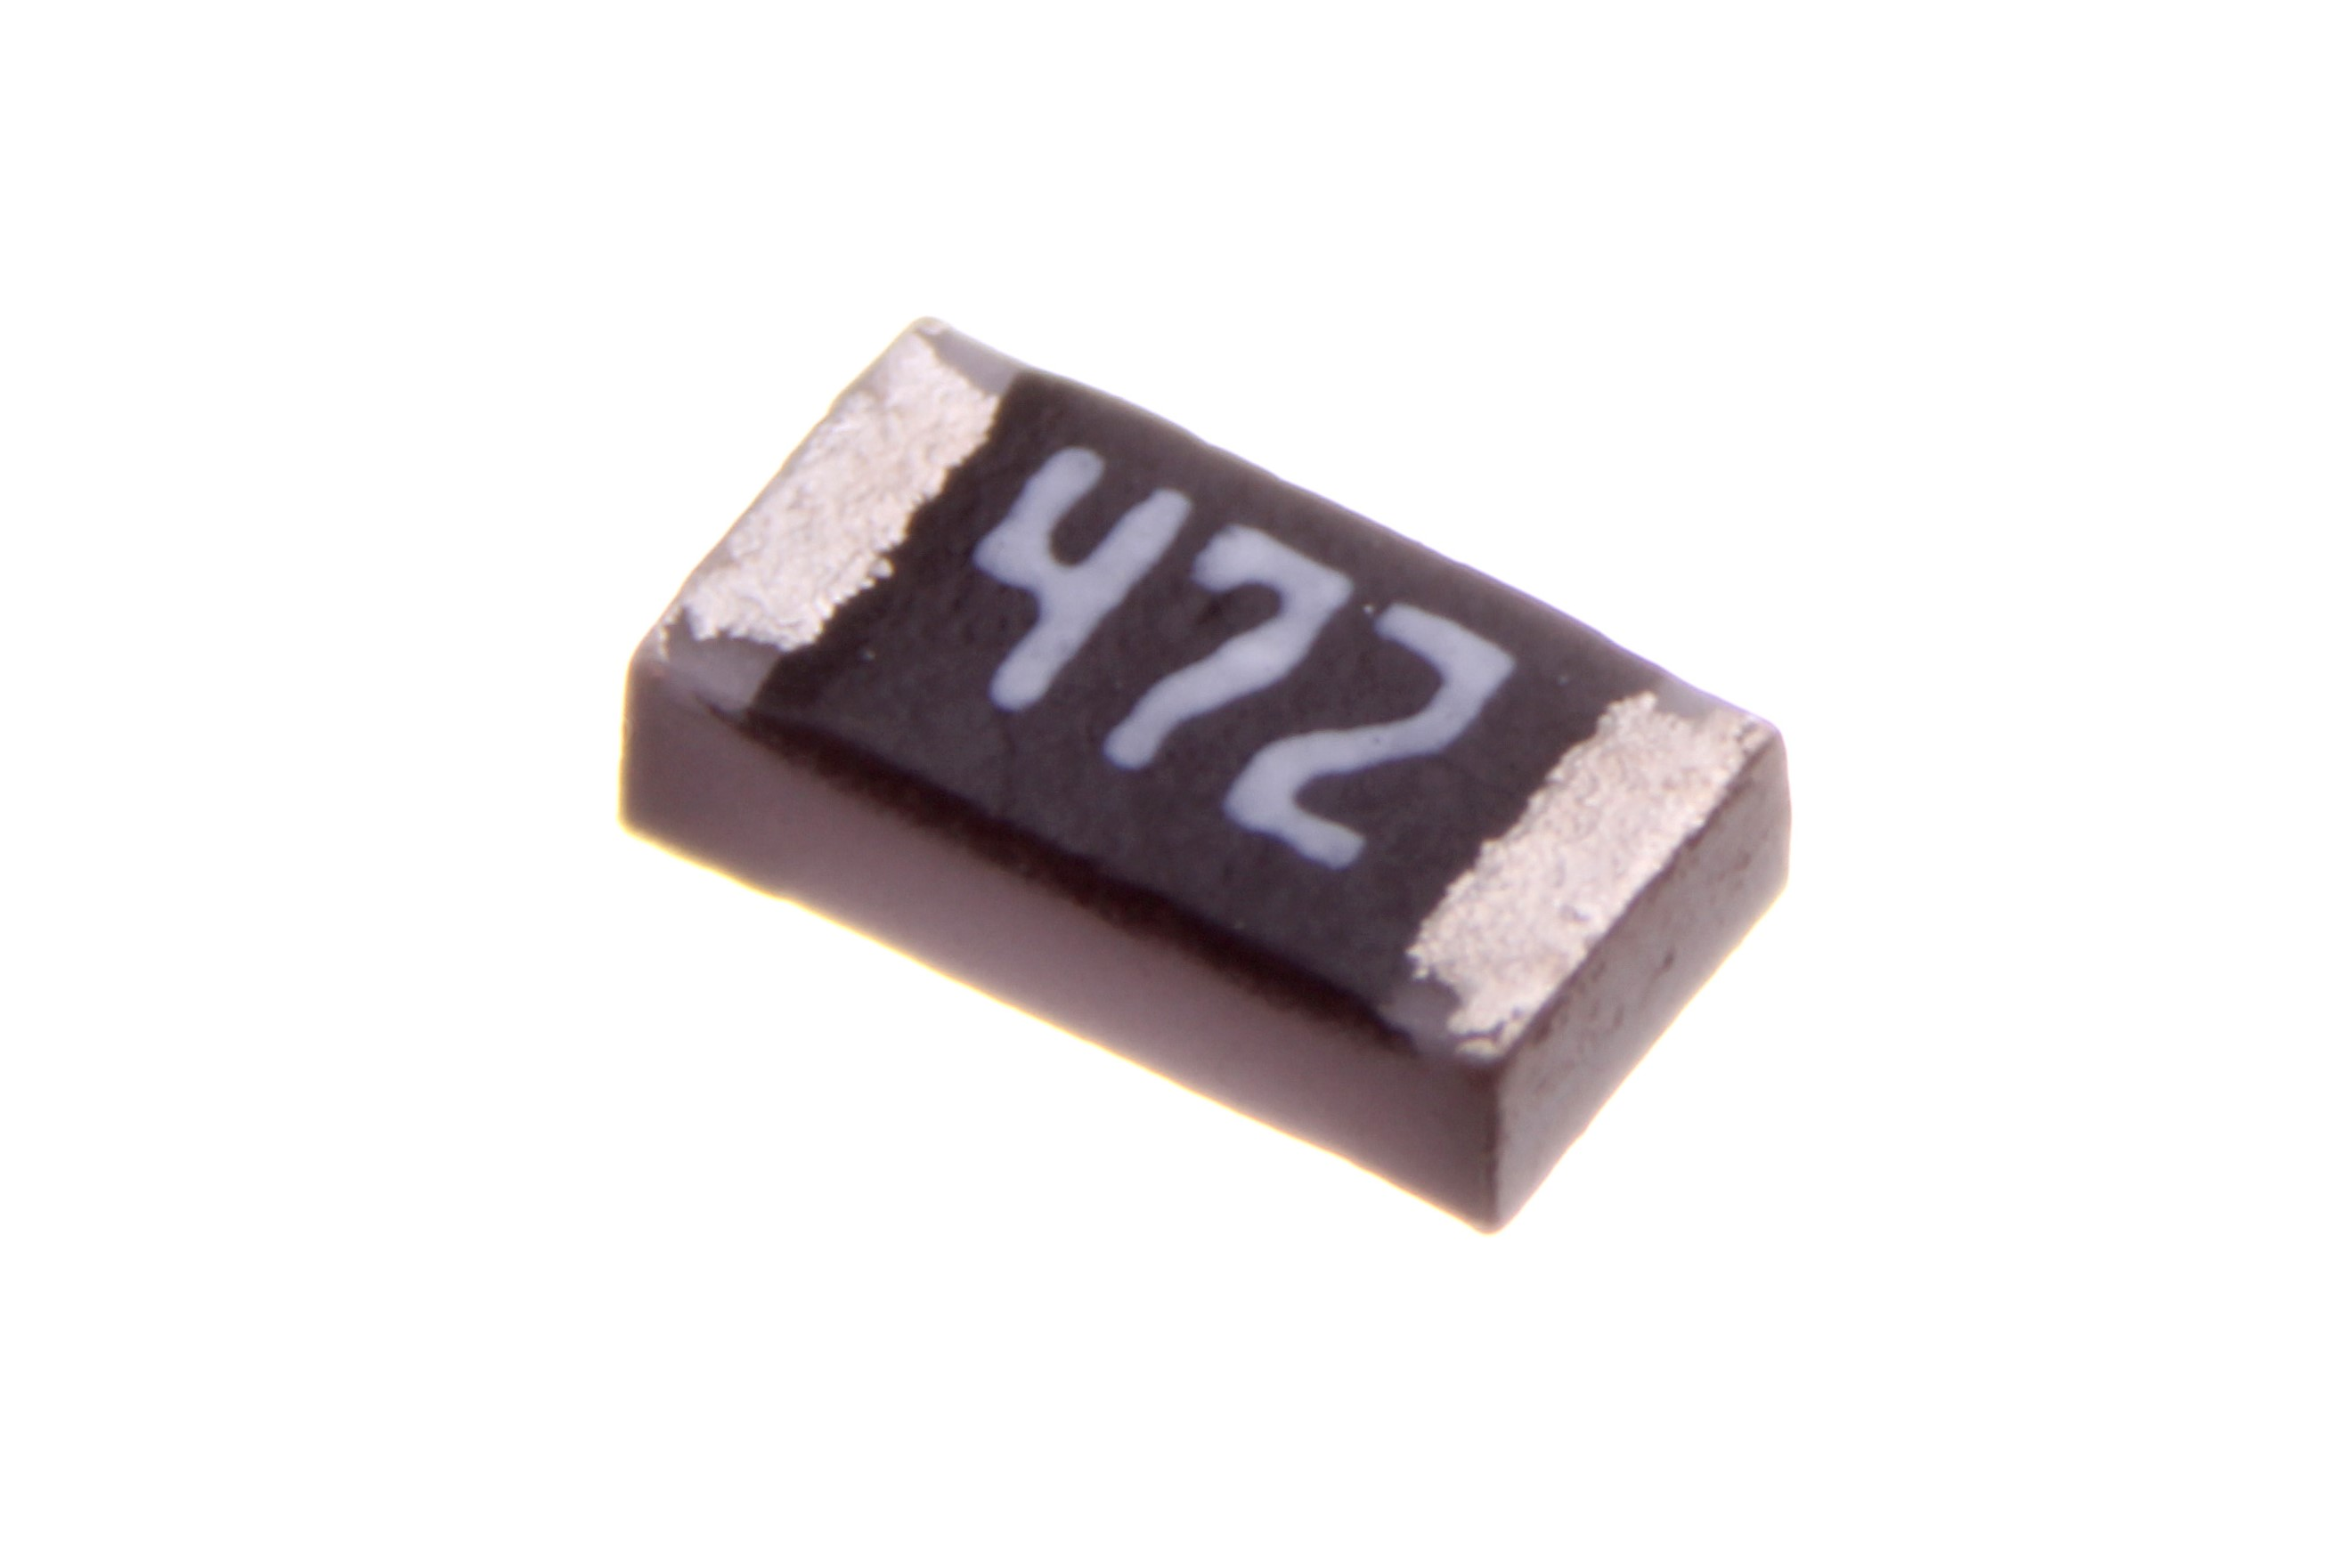
\includegraphics[width=0.75\textwidth]{img/4_7_kiloohm_SMD_0603_resistor.jpg}
	%\caption{Harvesting of the solar energy}
\end{figure}
$47 * 10^2~\Omega = 4,7~k\Omega$\\ 
\srctext{Image source: \url{https://commons.wikimedia.org/wiki/File:4.7_kiloohm_SMD_0603_resistor.jpg}}
\end{frame}

\begin{frame}
\frametitle{Součástky - SMD (surface mount device) - rezistor}    	
\begin{figure}[H]
	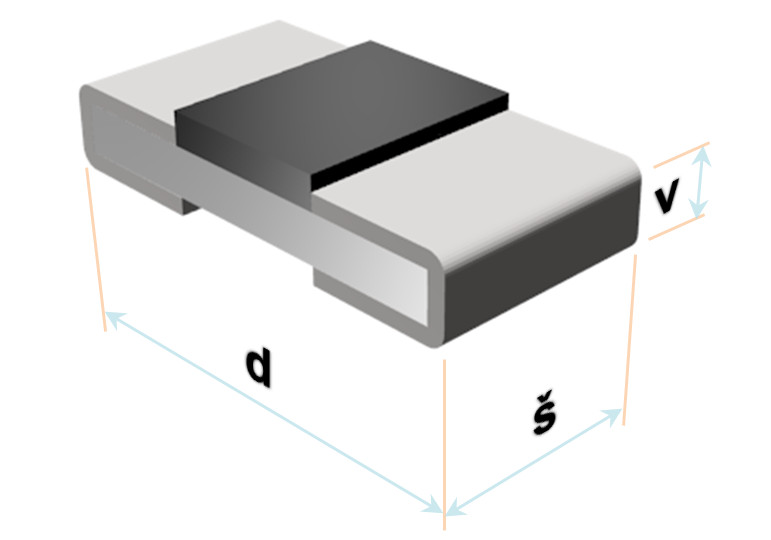
\includegraphics[width=0.77\textwidth]{img/Resistor_SMD.jpg}
	%\caption{Harvesting of the solar energy}
\end{figure}
\srctext{Image source: \url{https://commons.wikimedia.org/wiki/File:Resistor_SMD.jpg}}
\end{frame}

\begin{frame}
\frametitle{Součástky - SMD (surface mount device) - rezistor}    	
\begin{figure}[H]
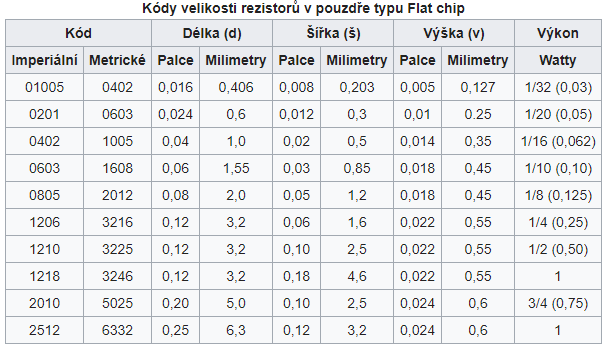
\includegraphics[width=0.92\textwidth]{img/Velikosti_SMD_soucastek.PNG}
%\caption{Harvesting of the solar energy}
\end{figure}
\srctext{Image source: \url{https://cs.wikipedia.org/wiki/SMT}}
\end{frame}

\begin{frame}
    \frametitle{Součástky - SMD (surface mount device) - IC}    	
        \begin{figure}[H]
            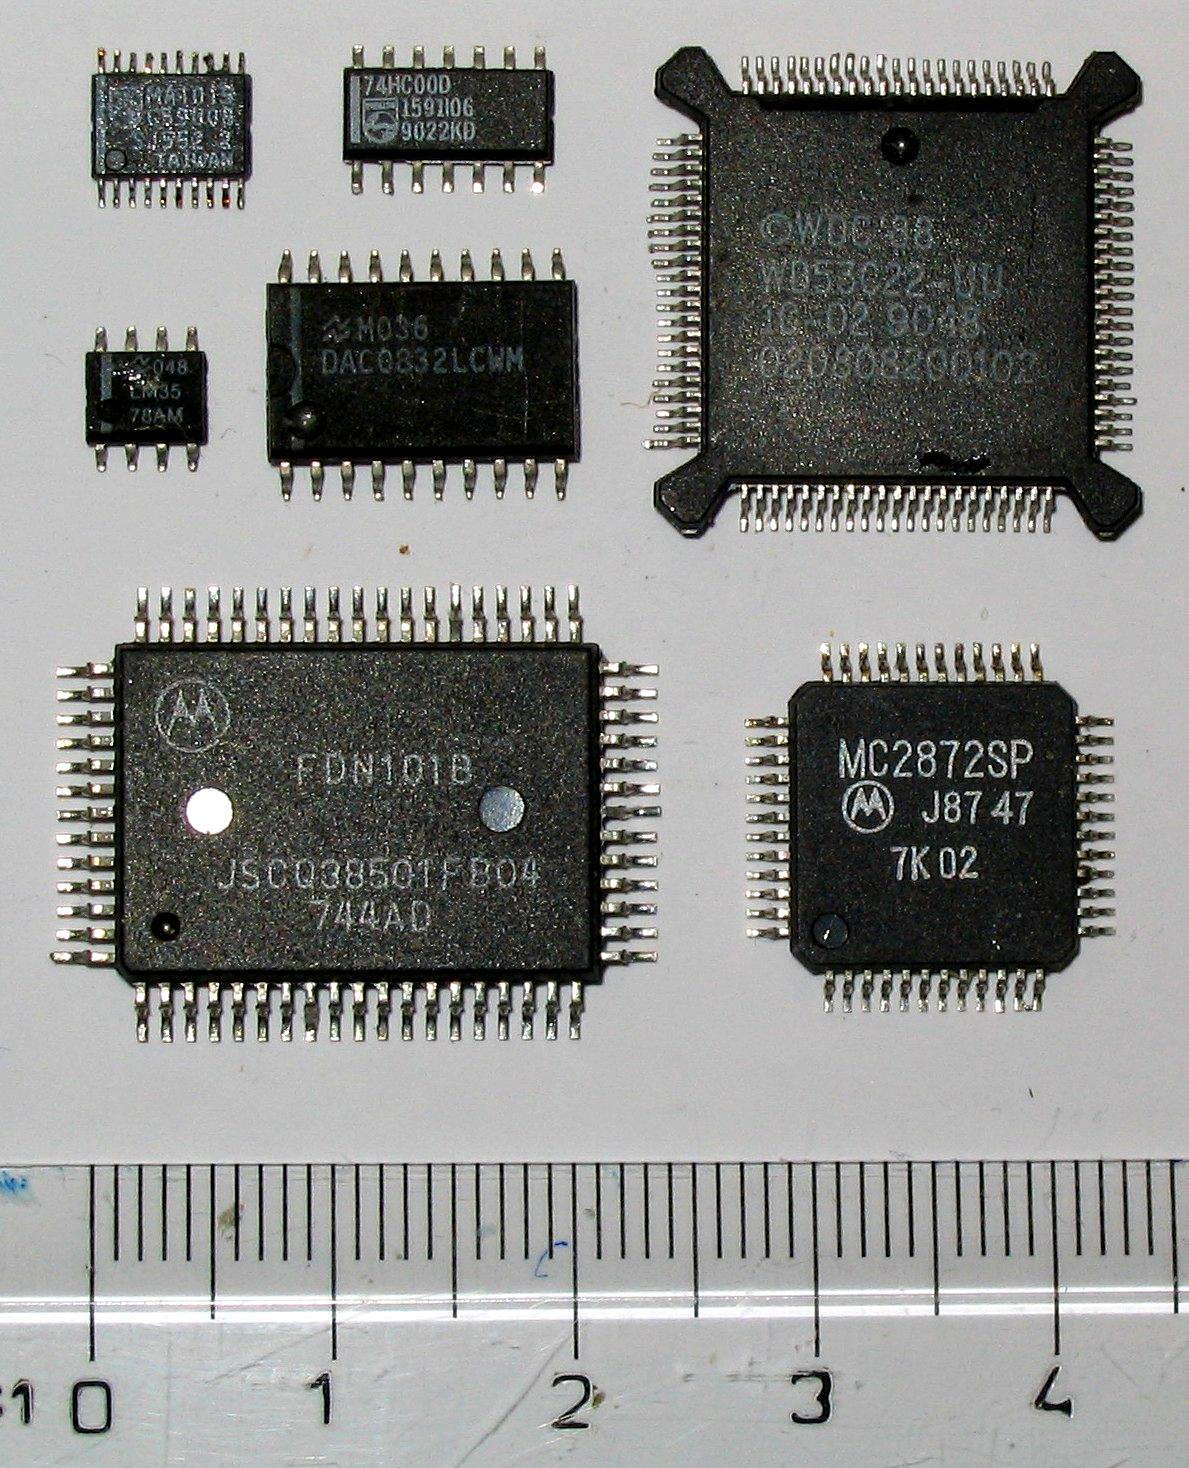
\includegraphics[width=0.45\textwidth]{img/Photo-SMDchips.jpg}
            %\caption{Harvesting of the solar energy}
       	\end{figure}
    \srctext{Image source: \url{https://commons.wikimedia.org/wiki/File:Photo-SMDchips.jpg}}
\end{frame}

\begin{frame}
\frametitle{Deska plošných spojů (DPS) / Printed circuit board (PCB)}    	
\begin{figure}[H]
	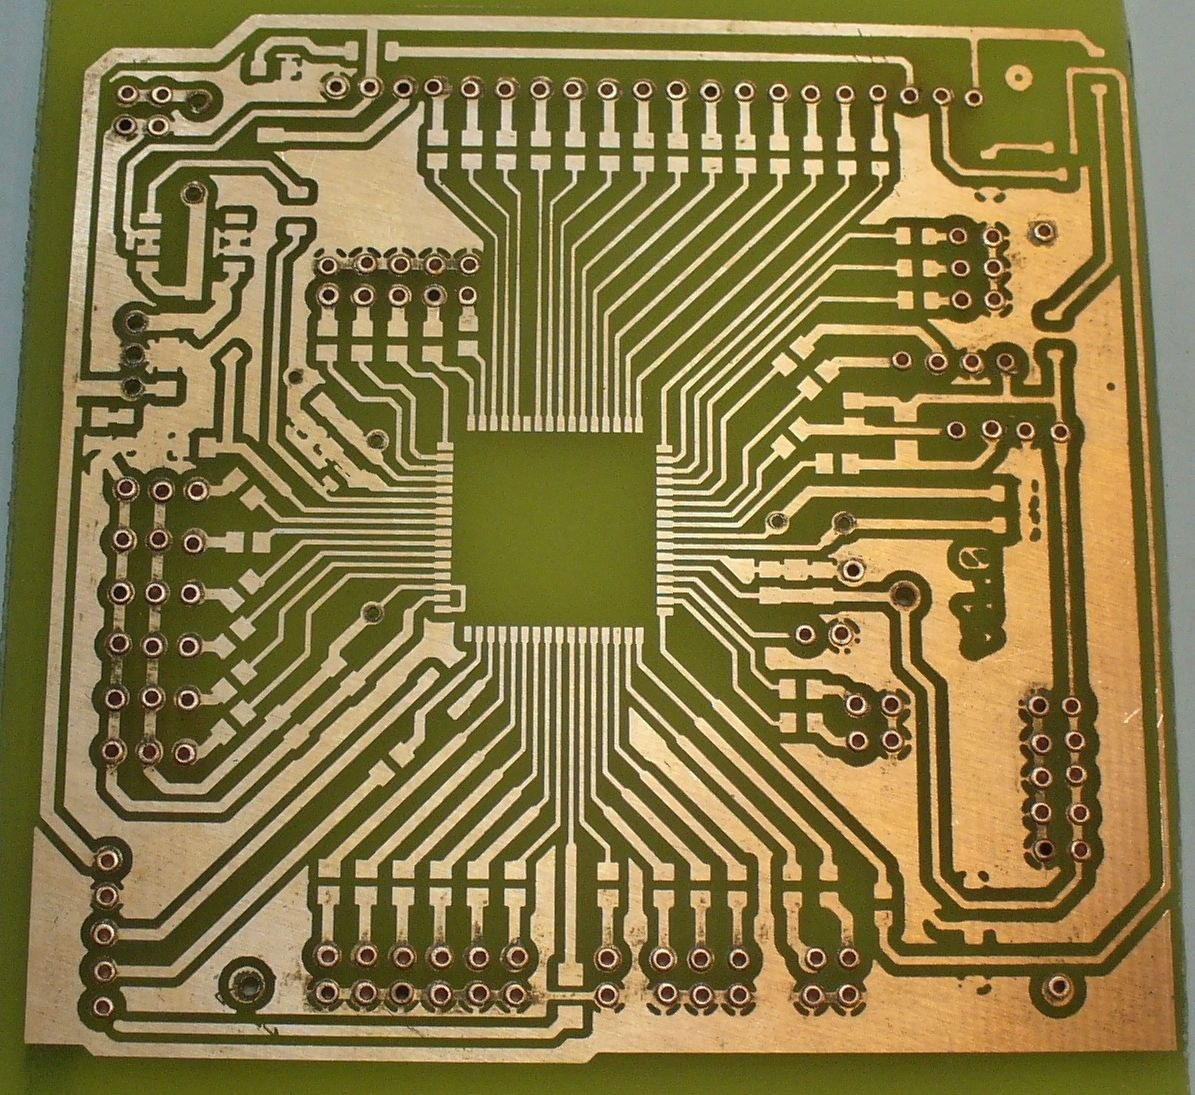
\includegraphics[width=0.62\textwidth]{img/dps_cesty.jpg}
	%\caption{Harvesting of the solar energy}
\end{figure}
\end{frame}


\begin{frame}
\frametitle{Deska plošných spojů (DPS) / Printed circuit board (PCB)}    	
\begin{figure}[H]
	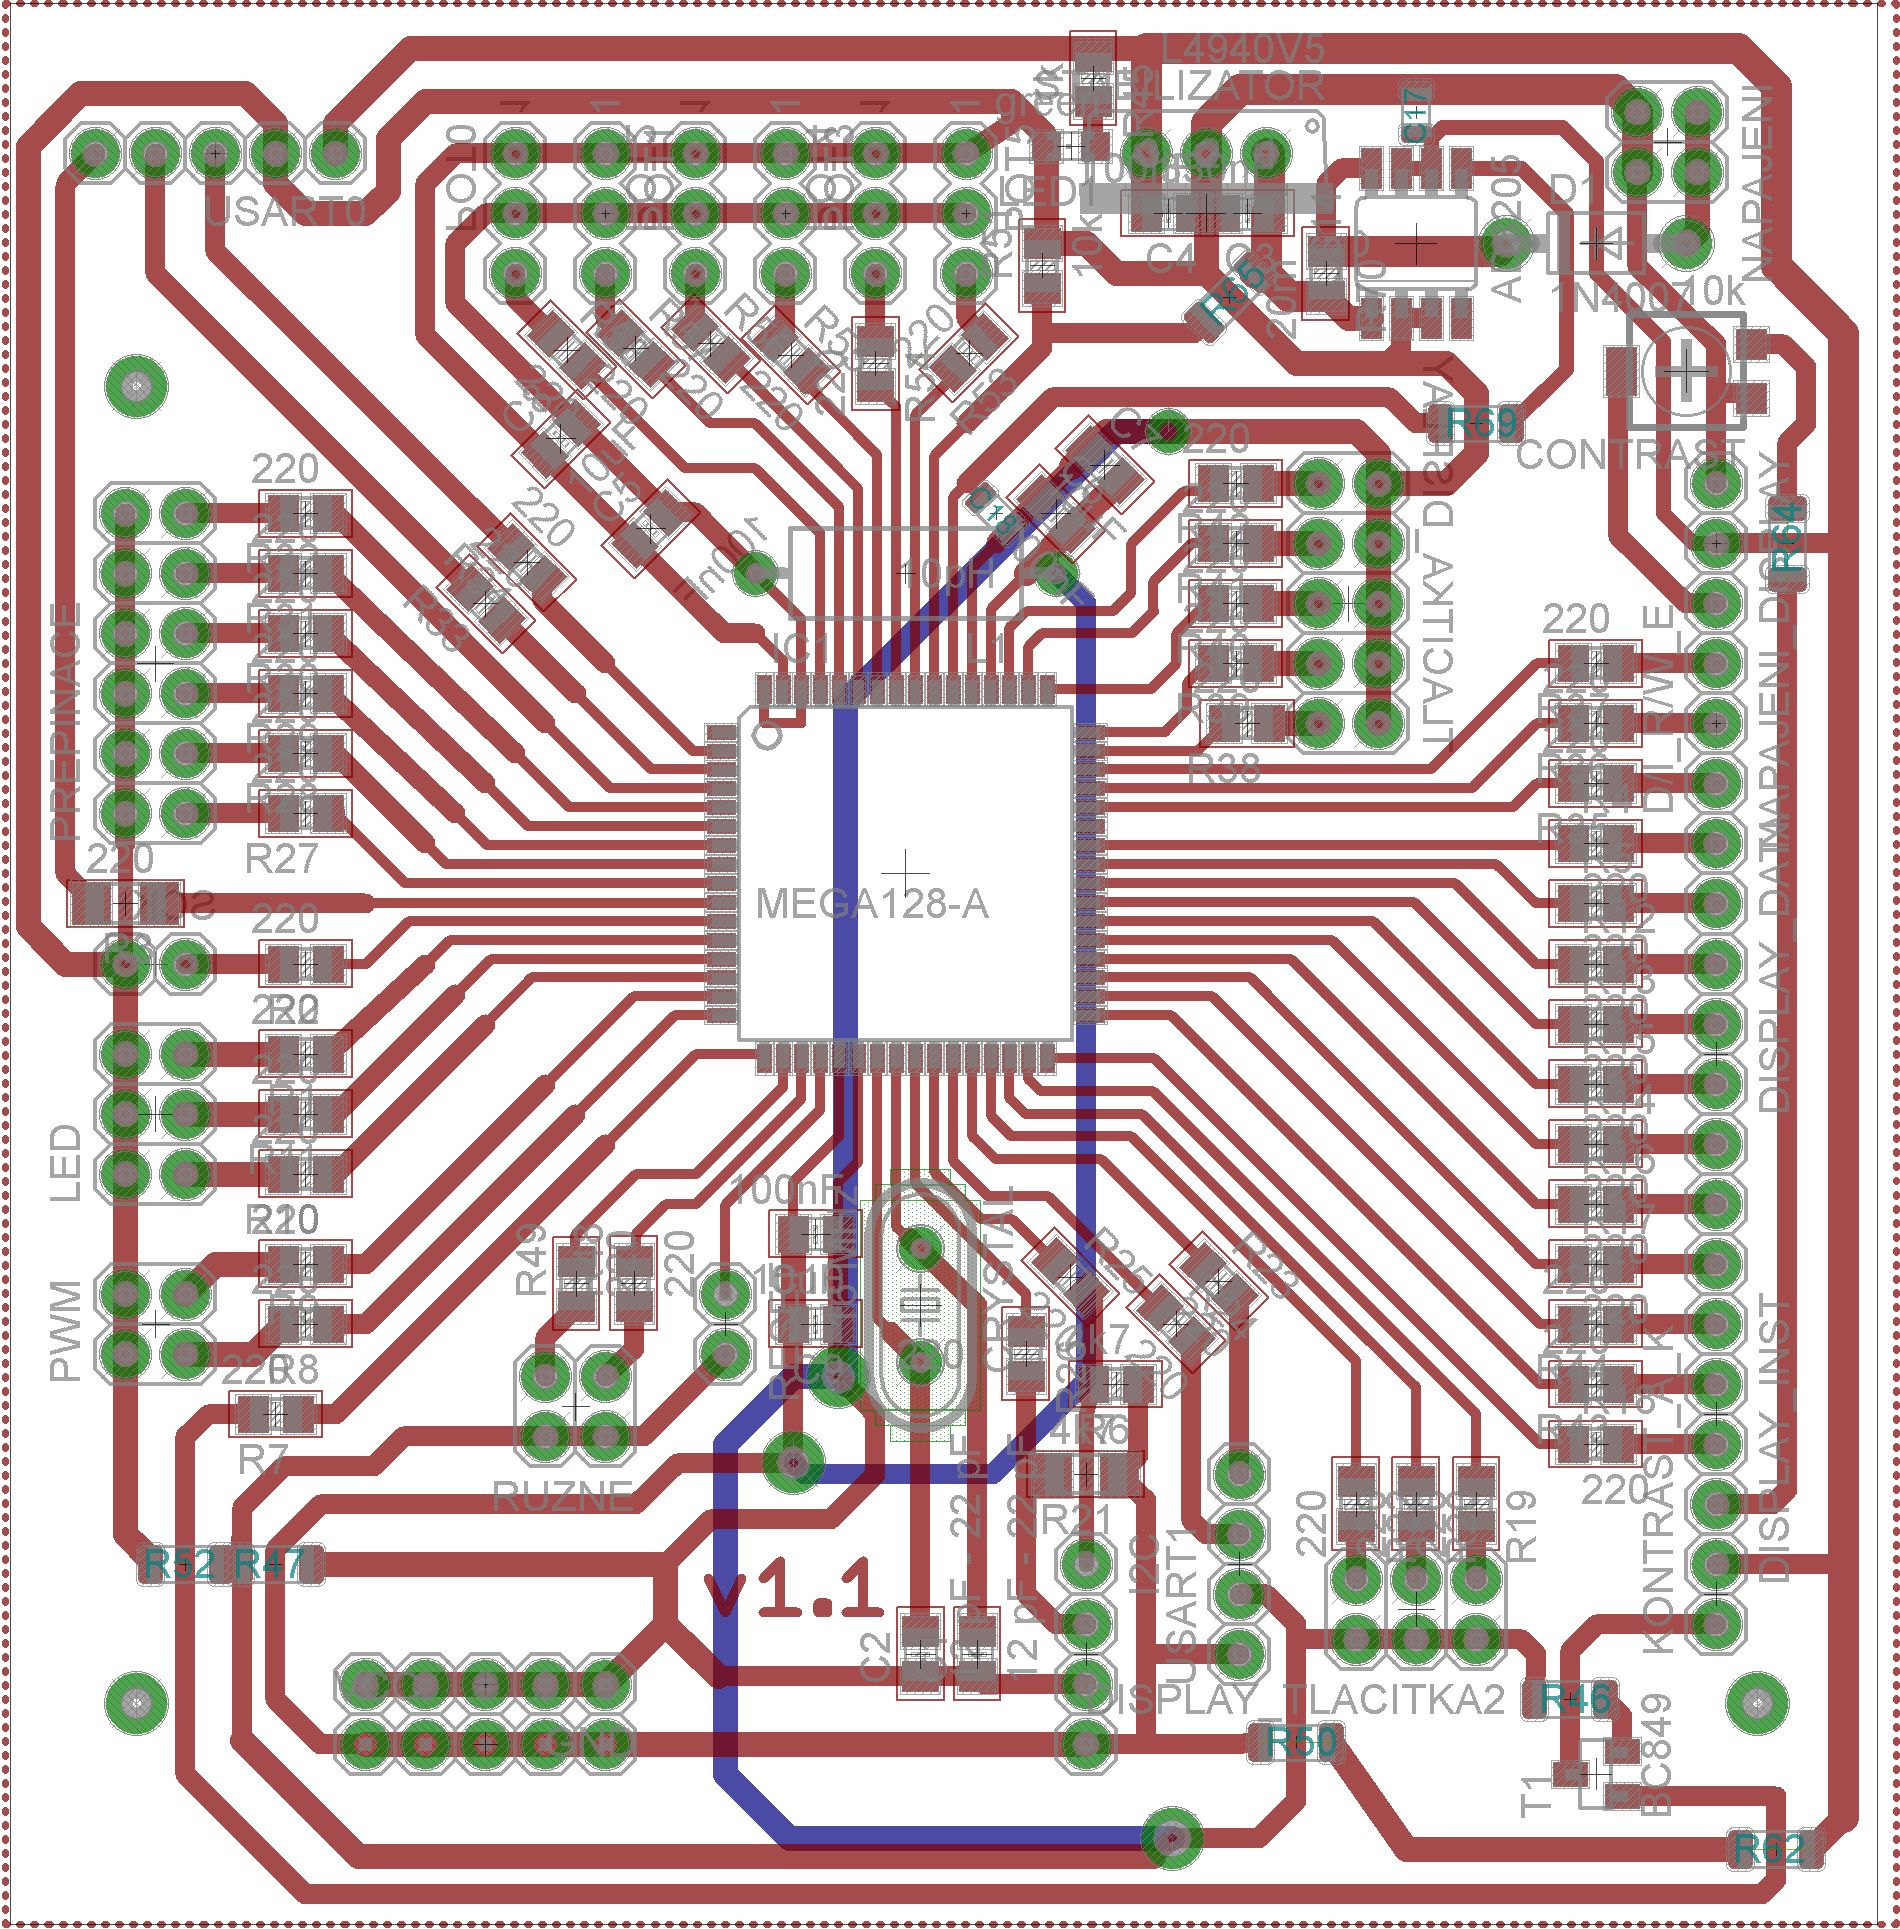
\includegraphics[width=0.57\textwidth]{img/transmit_b.jpg}
	%\caption{Harvesting of the solar energy}
\end{figure}
\end{frame}





\begin{frame}
\frametitle{Deska plošných spojů (DPS) / Printed circuit board (PCB)}    	
\begin{figure}[H]
	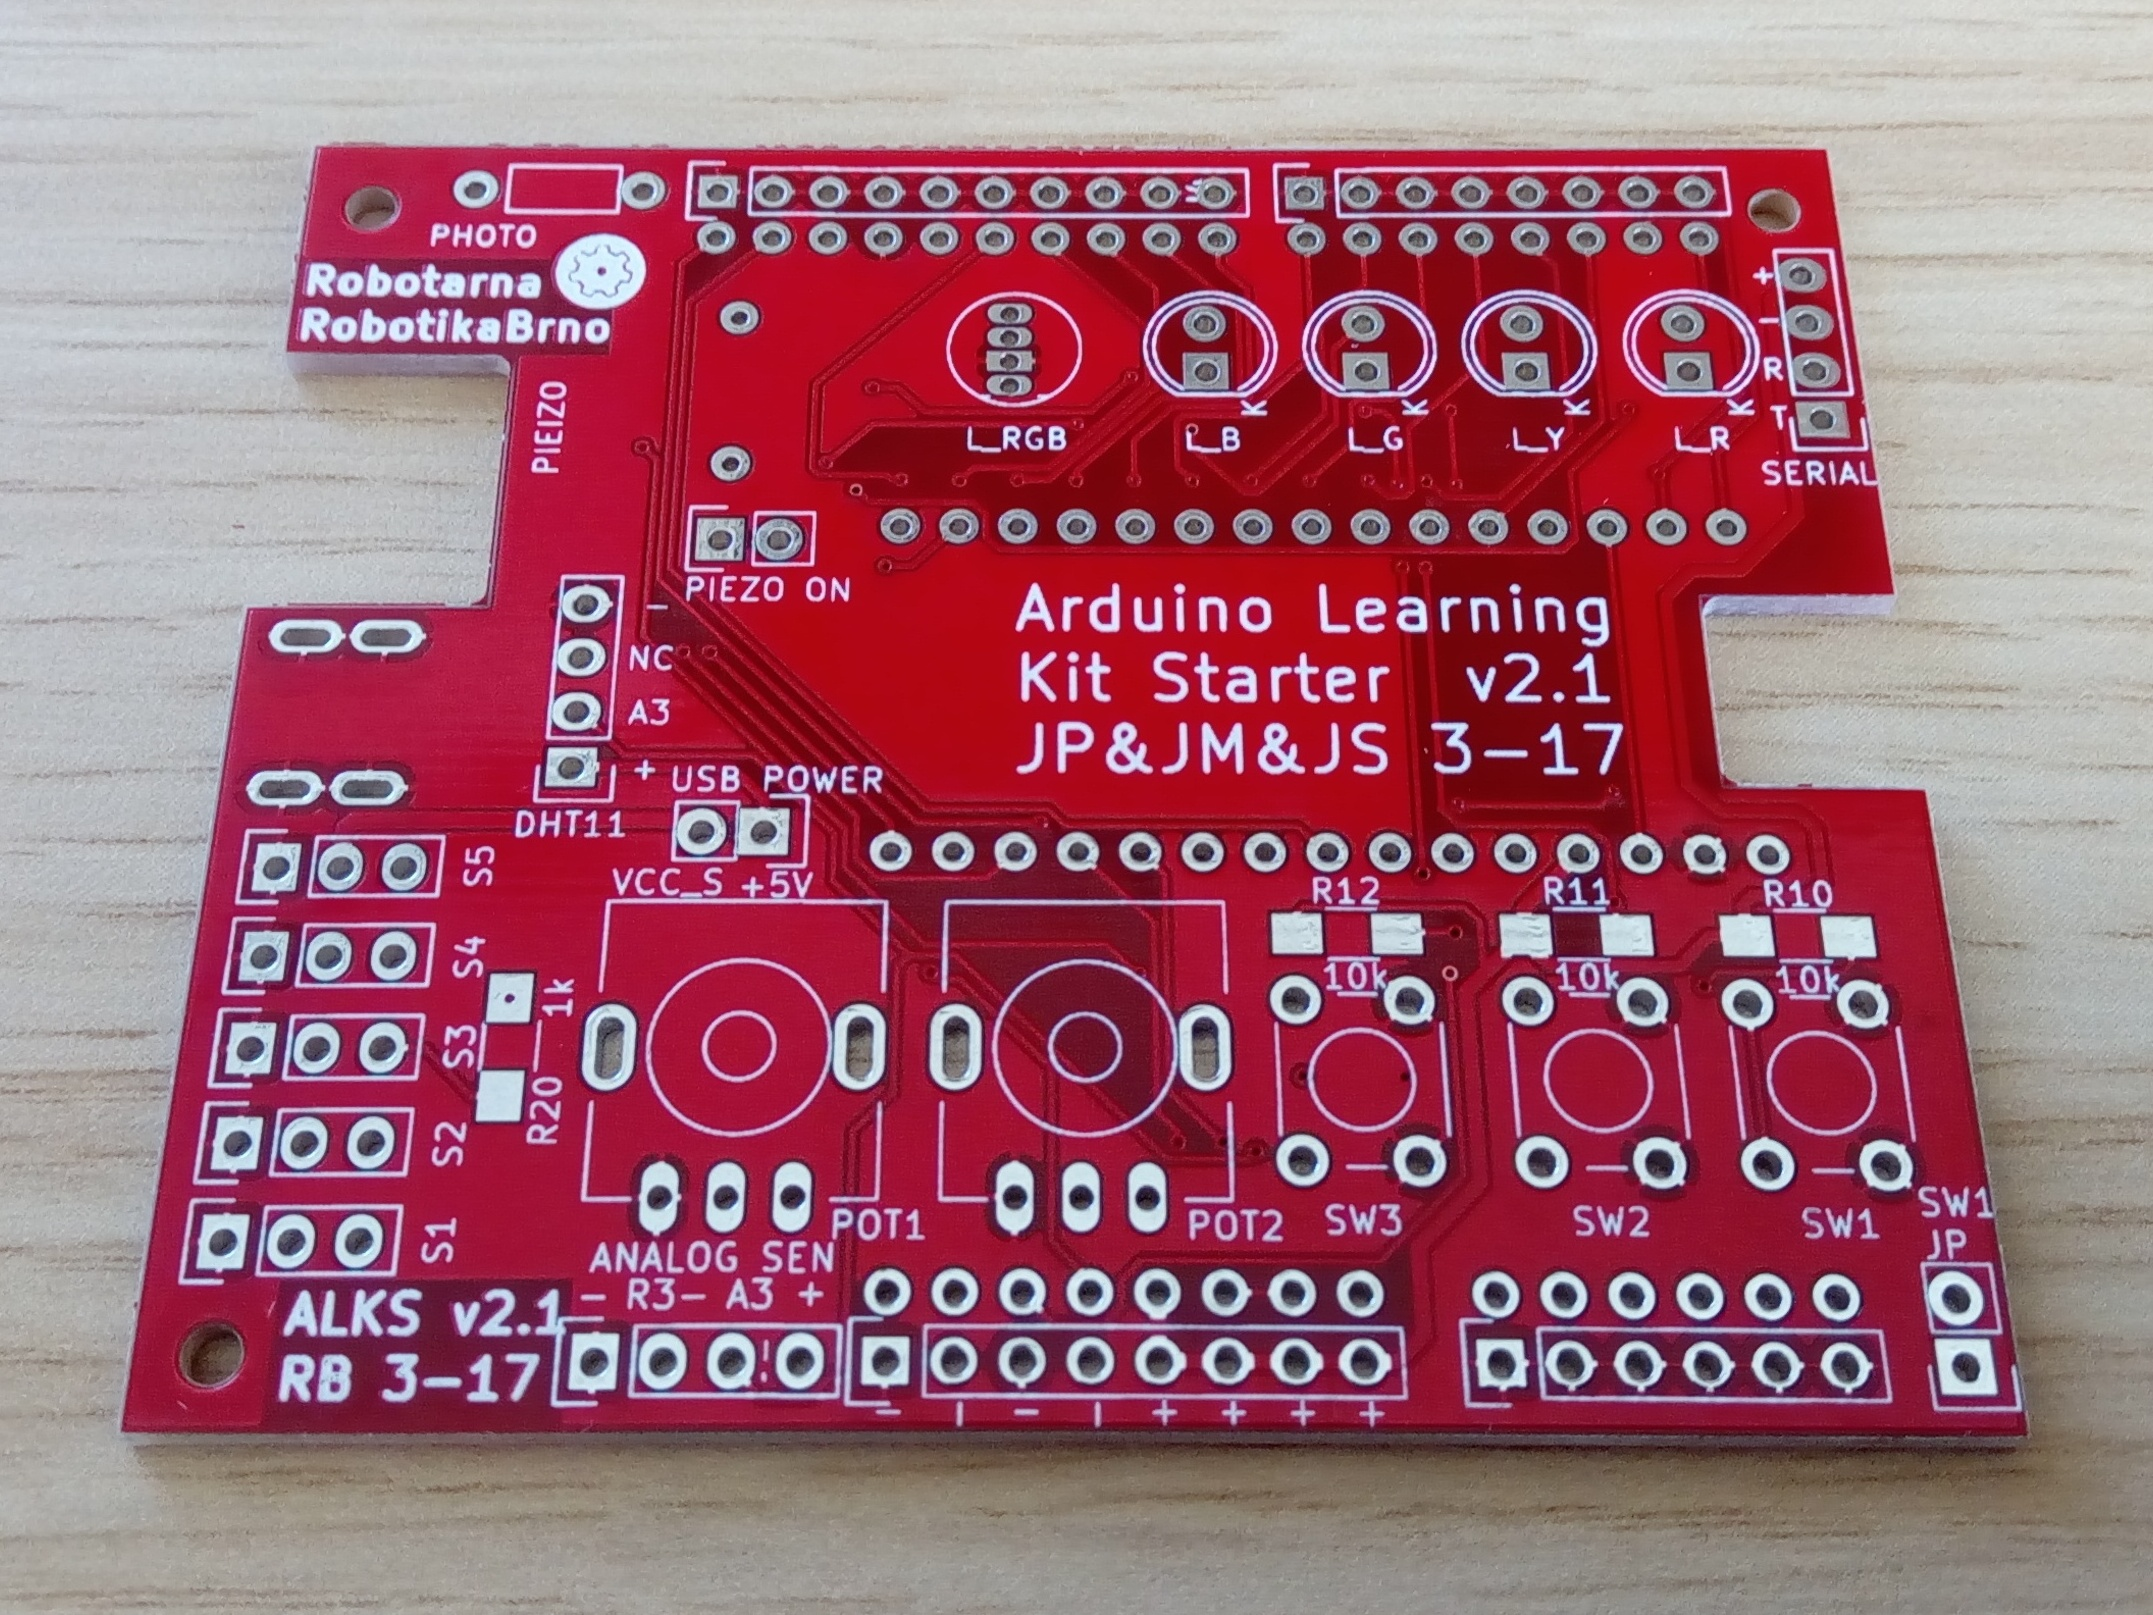
\includegraphics[width=0.7\textwidth]{img/ALKS_v2_1_1_01_top.JPG}
	%\caption{Harvesting of the solar energy}
\end{figure}
\srctext{Image source: \url{https://github.com/RoboticsBrno/ArduinoLearningKitStarter/releases}}
\end{frame}


\begin{frame}
\frametitle{Deska plošných spojů (DPS) / Printed circuit board (PCB)}    	
\begin{figure}[H]
	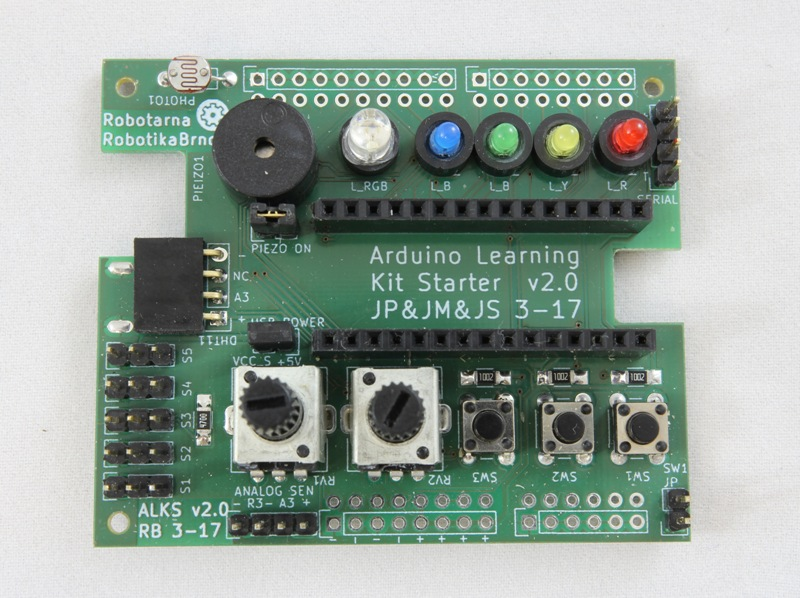
\includegraphics[width=0.74\textwidth]{img/ALKS_v2_0_2_01_top.JPG}
	%\caption{Harvesting of the solar energy}
\end{figure}
\srctext{Image source: \url{https://github.com/RoboticsBrno/ArduinoLearningKitStarter/releases}}
\end{frame}



\begin{frame}
\frametitle{Deska plošných spojů (DPS) / Printed circuit board (PCB)}    	
\begin{figure}[H]
	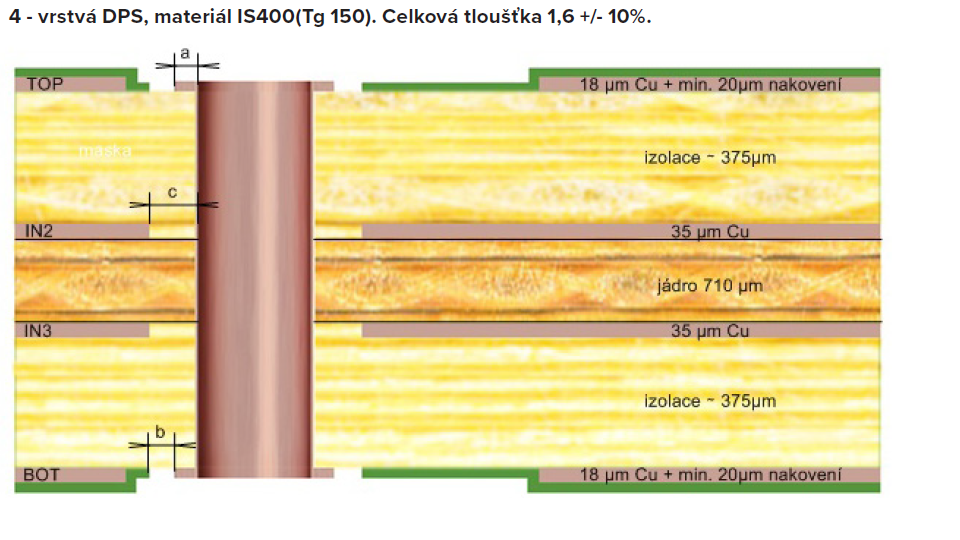
\includegraphics[width=0.96\textwidth]{img/Gatema_4-vrstva-DPS.png}
	%\caption{Harvesting of the solar energy}
\end{figure}
\srctext{Image source: \url{https://www.gatema.cz/files/file/Pool_kriteria.pdf}}
\end{frame}

\begin{frame}
\frametitle{Deska plošných spojů (DPS) / Printed circuit board (PCB)}    	
\begin{figure}[H]
	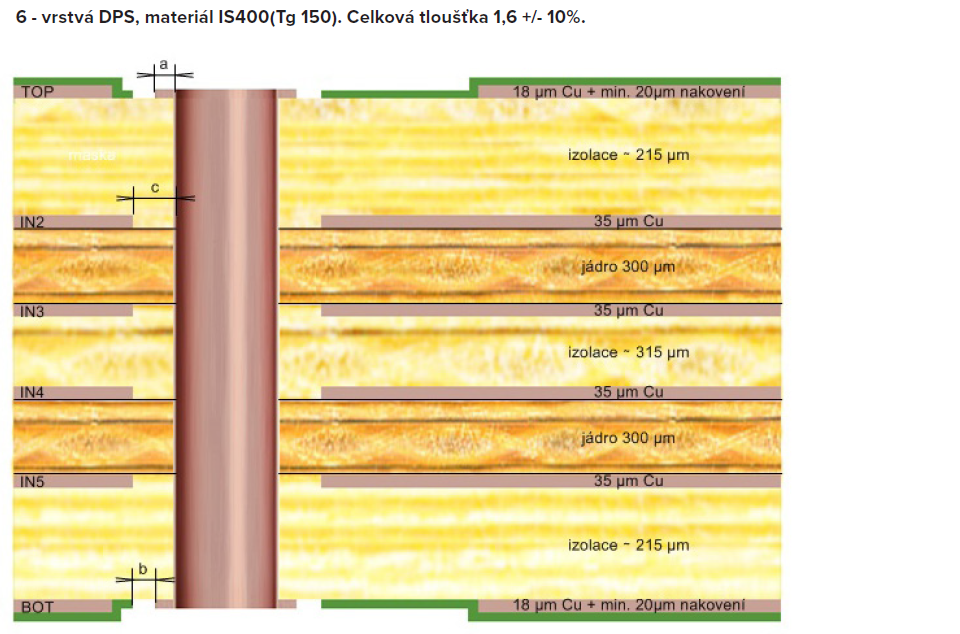
\includegraphics[width=0.82\textwidth]{img/Gatema_6-vrstva-DPS.png}
	%\caption{Harvesting of the solar energy}
\end{figure}
\srctext{Image source: \url{https://www.gatema.cz/files/file/Pool_kriteria.pdf}}
\end{frame}



%https://cs.wikipedia.org/wiki/SMT

\begin{frame}[fragile]
	\vfill
    \begin{center}
        {\huge Děkuji za pozornost}
	\end{center}
	\vfill
\end{frame}


\end{document}

